\documentclass[english]{article}
\usepackage[italian]{babel} 
\usepackage[T1]{fontenc}
\usepackage[utf8x]{inputenc}
\usepackage{float}
\usepackage{graphicx}
\makeatletter
\usepackage[a4paper,top=2cm,bottom=2cm,left=2cm,right=2cm]{geometry}
\usepackage{enumitem}
\usepackage{subfig}
\usepackage{amsthm}
\usepackage{amsmath}
\usepackage{epstopdf}
\usepackage{fancyhdr}
\usepackage{booktabs,array}
\newcommand*{\eacc}{\MakeUppercase{è }}

% Pacchetto per la gestione del testo colorato
\usepackage{color}

% Pacchetto che permette l'inserimento di codice Matlab formattato
\usepackage{listings} % inserisce listati di programmi
\definecolor{commenti}{rgb}{0.13,0.55,0.13}
\definecolor{stringhe}{rgb}{0.63,0.125,0.94}
\lstloadlanguages{Matlab}
\lstset{% general command to set parameter(s)
framexleftmargin=4mm,
frame=single,
keywordstyle = \color{blue},% blue keywords
identifierstyle =, % nothing happens
commentstyle = \color{commenti}, % comments
stringstyle = \ttfamily \color{stringhe}, % typewriter type for strings
showstringspaces = false, % no special string spaces
emph = {for, if, then, else, end},
emphstyle = \color{blue},
firstnumber = 1, % numero della prima linea
numbers =left, %  show number_line
numberstyle = \tiny, % style of number_line
stepnumber = 5, % one number_line after stepnumber
numbersep = 5pt,
language = {Matlab}, % per riconoscere la sintassi matlab
extendedchars = true, % per abilitare caratteri particolari
breaklines = true, % per mandare a capo le righe troppo lunghe
breakautoindent = true, % indenta le righe spezzate
breakindent = 30pt, % indenta le righe di 30pt
}




\hyphenation{italian}
\lhead{Progettazione Sistemi di controllo}
\rhead{Homework 1}

%\linespread{1.3}

%\@ifundefined{showcaptionsetup}{}{%
% \PassOptionsToPackage{caption=false}{subfig}}
%\usepackage{subfig}
\makeatother

\usepackage{babel}

\begin{document}
\begin{titlepage} 

\begin{center}
\begin{Large} \textbf{UNIVERSITA' DEGLI STUDI DI PADOVA} \\
 \end{Large} \vspace{1cm}

\begin{Large} \textsc{Corso di Robotica Autonoma }\end{Large}
\par\end{center}

\begin{center}
\begin{Large}\textsc{Esperienza 2}\\
 \end{Large}
\par\end{center}

\begin{center}
\vspace{2cm}
\begin{figure}[!htb]
\centering 
\includegraphics[width=8cm]{unipd}\\
 
\end{figure}

\par\end{center}

\begin{center}
\vspace{2cm}
 \begin{Large}
 GRUPPO 11: \\
 Marco Bertagnoli \\ 
 Matteo Mastellaro \\ 
 Angelo Trevisol\\
 \end{Large} \vspace{2cm}
 \begin{Large} Anno Accademico 2015-2016 \end{Large} 
\par\end{center}

\end{titlepage}

\tableofcontents
\newpage

\section{Introduzione} 
Il laboratorio di $Intelligent$ $Autonomous$ $Systems$ $Laboratory$ $(IAS$-$Lab)$ di Padova è fornito di un braccio manipolatore Universal Robot UR10, dotato di 6 giunti \textit{revolute}, comandato da un'interfaccia utente grafica su schermo touch screen da 12 pollici, montato su una piattaforma statica. Esso viene utilizzato sia per la didattica, sia per argomenti di ricerca che prevedono l'utilizzo del manipolatore per eseguire operazioni di pick and place, ad esempio interagendo con la portiera di una macchina posizionata adiacentemente ad esso. A tal proposito questa esperienza affronta uno dei primi sottoproblemi riscontrabili, ovvero quello di identificare un oggetto, e di conseguenza porre l'end-effector in una certa posa rispetto all'oggetto identificato. Per far fronte a ciò, il manipolatore si avvale di una coppia di videocamere in configurazione stereo, posizionate in corrispondenza dell'end-effector. In altre parole, se si pensa al manipolatore come sistema da controllare, si andrà ad sfruttare l'uscita video delle camere come feedback, per elaborare il controllo del manipolatore, in questo caso il movimento dell'end-effector. 


\begin{figure}[!h]
\centering
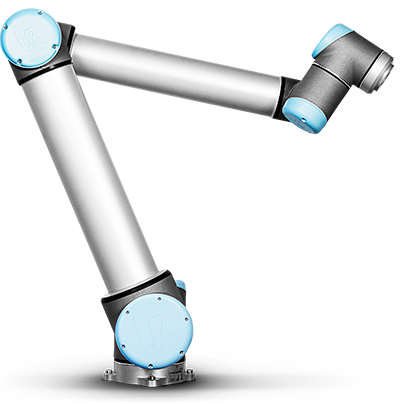
\includegraphics[width=0.35\textwidth]{ur10}
\caption{Universal Robot UR10.}
\label{fig:ur10}
\end{figure}

\section{Obiettivi e Procedimento}
L'obiettivo di tale esperienza è dunque quello di identificare un oggetto (nello specifico una lattina di alluminio) attraverso un matching tra le informazioni dalle telecamere e un pattern predefinito, conosciuto a priori (una istantanea della lattina). Il tutto viene svolto in simulazione sfruttando i seguenti:
\begin{itemize}
\item \textit{Gazebo}, plugin che inizializza un nodo ROS con cui è possibile comunicare attraverso i comandi forniti dallo stesso ambiente ROS. Con quest'ultimo, è stato ricreato l'ambiente in cui opera il manipolatore in laboratorio (Figura \ref{fig:gazebo}).
\item \textit{MoveIt!}, una user friendly utility disponibile nel software \textit{rviz}, che fornisce strumenti di motion planning, manipolazione, percezione 3D, cinematica, controllo e navigazione; in questa esperienza verrà utilizzata per pianificare il movimento del manipolatore.
\end{itemize}
La necessità di usare i precedenti software nasce dall'esigenza di voler implementare e testare l'efficacia degli algoritmi in ambiente simulativo. Questo permette appunto di potersi focalizzare sulla parte progettuale, senza doversi imbattere da subito in problemi tecnici che derivano dall'interfacciamento con il sistema reale, oltre al fatto che non si sottopone quest'ultimo al rischio di eventuali errori di implementazione. Tale esperienza si pone dunque il raggiungimento dei seguenti obiettivi:
\begin{itemize}
\item Trovare un template appropriato che rappresenti adeguatamente l'oggetto per entrambe le camere destra e sinistra
\item Cambiare leggermente la posa dell'oggetto
\item Usare un algoritmo di feature matching per stimare la nuova posa dell'oggetto 
\item Utilizzare la cinematica inversa per ricavare una configurazione del robot valida
\item Utilizzare \textit{MoveIt!} per pianificare il moto del robot evitando gli ostacoli
\item Ripetere finchè la posa delle camere rispetto all'oggetto sia all'interno di una determinata tolleranza.
\end{itemize}

Per raggiungere questi obiettivi, il nodo ROS \textit{pose} \textit{estimation} offre 3 utili servizi:
\begin{enumerate}
\item Servizio \textit{InitCameras}, permette di inizializzare le informazioni di sistema. In particolare qui vengono forniti i parametri intrinseci delle due camere e i reference frames \textit{end-effector} e \textit{robot base}.   
\item Servizio \textit{TrainPose}, consente di effettuare un train della posa desiderata dell'end-effector rispetto all'oggetto. In input vengono forniti i keypoints estratti dalle camere destra e sinistra, mentre come output verranno forniti le posizioni 3D dei keypoints di ingressi, ottenuti attraverso triangolazione, e la desiderata end-effector transformation calcolata da ciascuna delle due camere.
\item Servizio \textit{QueryPose} restituisce la nuova posa dell'end-effector, ricavata sulla base di una corrispondenza tra una serie di keypoints e quelli forniti durante la fase di training.
%sulla base di una serie di keypoints con i quali è stata trovata corrispondenza con quelli forniti durante la fase di training. 

\end{enumerate}
Una volta eseguita la fase di inizializzazione è necessario definire la posa relativa alla lattina che si vuole far assumere all'end effector, e in questo caso si è optato per una posizione lungo sull'asse congiungente la lattina con la base del manipolatore, in modo da agevolare la fase di detection dell'oggetto. Con l'end effector posizionato in questo modo, attraverso un algoritmo di feature matching, si individuano le corrispondenze tra i keypoints appartenenti alla lattina nelle immagini provenienti dalle due camere, questi dati vengono quindi elaborati dal servizio di \textit{pose training} in modo da stabilire una relazione tra la posizione tridimensionale dei punti appena individuati e l'end effector. A questo punto la lattina e/o l'end effector vengono spostati, si recuperano nuovamente i keypoints appartenenti alla lattina da una delle due camere e se almeno alcuni tra questi erano presenti anche nella fase di training con il servizio di \textit{pose query} è possibile calcolare la nuova posa dell'end effector in modo che la sua posizione rispetto alla lattina sia quella desiderata. Potrebbero essere necessarie più iterazioni della fase di \text{pose query} affnchè l'errore di posizionamento sia minore di un certo valore desiderato. Si noti che ad ogni iterazione l'end effector si avvicina sempre più alla posa desiderata rendendo sempre più semplice trovare corrispondenze tra i keyponts delle fasi di training e query.

\begin{figure}[!h]
\centering
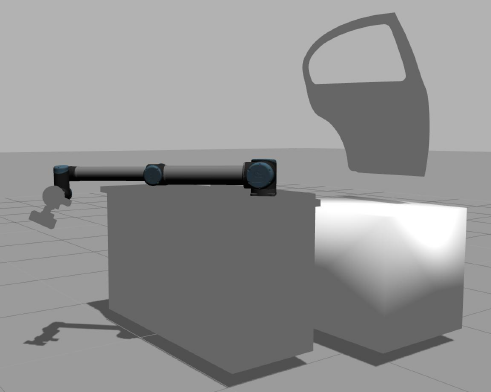
\includegraphics[width=0.35\textwidth]{gazebo}
\caption{Software di simulazione Gazebo.}
\label{fig:gazebo}
\end{figure}

\section{Implementazione}
Per portare a termine il procedimento descritto nella sezione precedente si sono implementati 3 nodi:
\begin{enumerate}
\item \textit{robot\_controller}: nodo che si occupa di avviare il servizio che permette di muovere il robot in una qualsiasi posizione raggiungibile.

\item \textit{Detector}: nodo che si occupa di trovare i matching tra template ed immagini destra e sinistra delle camere da usare poi nelle fasi di training e query.

\item \textit{move\_to\_object}: nodo che gestisce le chiamate ai due precedenti ed ai servizi di \textit{pose estimation}.
\end{enumerate}

\subsection{\textit{robot\_controller}}
Implementato nel file \textit{move\_robot.cpp} si occupa di avviare il servizio \textit{robot\_controller/move\_robot} definito nel file \textit{esperienza2/MoveUR.srv} e può essere lanciato attraverso il file \textit{robot\_controller.launch}. Questo servizio prende come ingresso la posizione e l'orientamento dell'end effector (\textit{\textbackslash ee\_link} frame) rispetto al frame \textit{\textbackslash world}, prova a pianificare una traiettoria dalla posizione attuale a quella desiderata  visualizzandola in $rviz$, se la posizione desiderata è raggiungibile muove il robot restituendo il valore booleano \textit{true}. Se la posizione non è raggiungibile si riprova a pianificare la traiettoria in quanto l'algoritmo non è deterministico e potrebbe giungere comunque ad una soluzione. Dopo cinque tentativi falliti il robot non viene mosso e si restituisce \textit{false}. Come algoritmo di motion planning si è scelto di utilizzare OMPL in quanto si è visto dare buoni risultati se si pongono dei limiti di movimento per i giunti del robot. È sconsigliabile utilizzarlo in caso di giunti non limitati, in quanto le soluzioni aggiungono vistosi movimenti non necessari del manipolatore.

\subsection{\textit{Detector}}
Implementato nel file \textit{detection\_node\_Flann.cpp} come libreria. Il costruttore prende in ingresso il path all'immagine di template (Figura \ref{fig:template}) ed i topic delle due camere. Si occupa di calcolare keypoints e matching da fornire ai servizi di query e train. Keypoints e descrittori sono calcolati con l'algoritmo SURF mentre si utilizza il FLANN matcher per ottenre le corrispondenze tra varie immagini. Oltre al costruttore sono disponibili due metodi pubblici:
\begin{enumerate}
\item \textit{std::vector<opencv\_apps::Point2DArray> Detector::TrainMatches(int kp\_num = 15,\\ int max\_iteration\_number = 100)}
\\ permette di ottenere i due vettori di keypoints provenienti dall'immagine di sinistra e destra da utilizzare per la fase di training. Riceve in ingresso il numero di keypoints da recuperarare dalle due immagini ($kp\_num$) ed il numero massimo di iterazioni che può compiere per effettuare la ricerca ($max\_iteration\_number$). Il metodo esegue la seguente serie di istruzioni:
	\begin{enumerate}
	\item Recupera le immagini dalle due camere e ne calcola keypoints e descrittori.
	\item Esegue il match tra le due immagini.
	\item Estrae i keypoints e relativi descrittori trovati in entrambe le immagini e riesegue il match con l'immagine di template in modo da selezionare solamente quelli appartenenti alla lattina.
	\item Salva i keypoints e relativi descrittori per cui si è trovato un match nel template controllando che non ci siano duplicati.
	\item Se il numero di keypoints trovati è minore di $kp\_num$ riparte dall'inizio aggiungendo ad ogni iterazione i keypoints trovati.
	\item una volta raggiunti i $kp\_num$ keypoints o $max\_iteration\_number$ iterazioni salva i descrittori e keypoints trovati in modo che possano essere utilizzati nella successiva fase di query, visualizza le corrispondenze trovate (Figure \ref{fig:train}) e restituisce un vettore riempito con i due array contenenti i keypoints delle immagini di sinistra e destra rispettivamente. Keypoints corrispondenti avranno lo stesso indice nei due vettori.
	\end{enumerate} 

\item \textit{std::vector<opencv\_apps::Point2DArray> Detector::QueryMatches(int kp\_num = 10, bool use\_camera\_left = true, int max\_iteration\_number = 100)} 
\\ permette di ottenere i keypoints da una delle due camere corrispondenti alla fase di training per essere utilizzati nella fase di pose query. Riceve in ingresso il numero di keypoints da recuperarare dalle due immagini ($kp\_num$), il numero massimo di iterazioni che può compiere per effettuare la ricerca iniziale dei keypoints ($max\_iteration\_number$) ed infine un valore booleano che permette di specificare da che camera recuperarli ($use\_camera\_left$). L'uscita è invece composta da un vettore contenente due array, il primo contiene i keypoints trovati ed il secondo una mappa di correlazione che indica a che indice del vettore di training corrispondono. Per semplicità la mappa di correlazione è espressa come $opencv\_apps::Point2DArray$, i valori $x$ ed $y$ del punto $2D$ sono uguali ed indicano l'indice in cui si trova il keypoint corrispondente nel vettore utilizzato per la fase di training. Il numero di keypoints restituito è solitamente minore del valore $kp\_num$ in quanto non è detto che tutti i keypoints trovati siano stati rilevati anche nella precedente fase di training. Il metodo esegue la seguente serie di operazioni:
	\begin{enumerate}
	\item Recupera l'immagine dalla camera indicata e ne calcola keypoints e descrittori.
	\item Esegue il matching con l'immagine di template per selezionare i soli punti della lattina (Figura \ref{fig:query_template}).
	\item Salva i keypoints trovati controllando che non ci siano duplicati.
	\item Se il numero di keypoints trovati è minore di $kp\_num$ riparte dall'inizio aggiungendo ad ogni iterazione le nuove scoperte.
	\item una volta raggiunti i $kp\_num$ keypoints o $max\_iteration\_number$ iterazioni esegue il match tra i punti trovati e quelli forniti nella fase di train.
	\item Dal match appena eseguito estrae i keypoints selezionati e le rispettive corrispondenze con l'array di training, visualizza il risultato (Figura \ref{fig:query_camera}) e restituisce in uscita i due vettori.	
	\end{enumerate}
\end{enumerate}

\begin{figure}[!h]
\centering
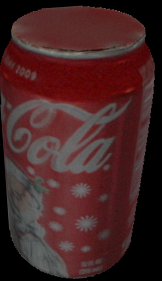
\includegraphics[width=0.15\textwidth]{template_lattina}
\caption{Immagine template per il riconoscimento della lattina.}
\label{fig:template}
\end{figure}

\begin{figure}[!h]
\centering
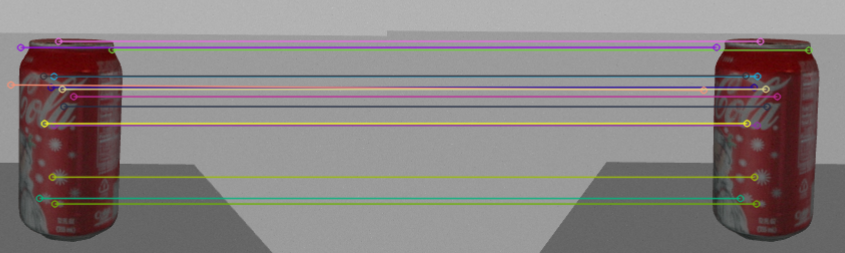
\includegraphics[width=0.7\textwidth]{train}
\caption{Risultato del matching tra le immagini delle camere destra e sinistra per la fase di training.}
\label{fig:train}
\end{figure}

\begin{figure}[!h]
\centering
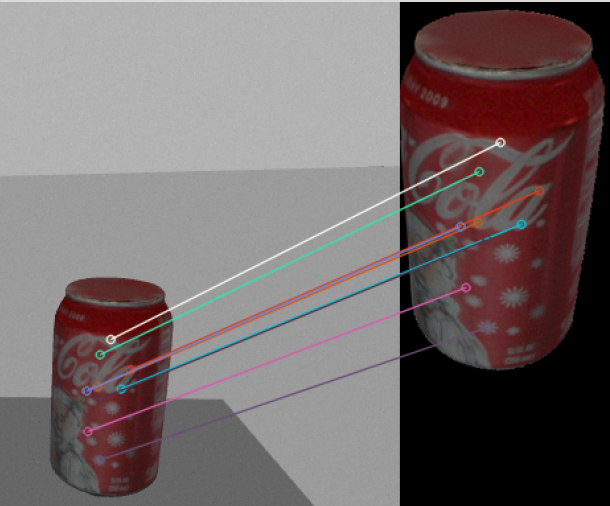
\includegraphics[width=0.35\textwidth]{template}
\caption{Risultato parziale della ricerca del matching tra i keypoints del template e dell'immagine della camera che si desidera utilizzare per la fase di training.}
\label{fig:query_template}
\end{figure}

\begin{figure}[!h]
\centering
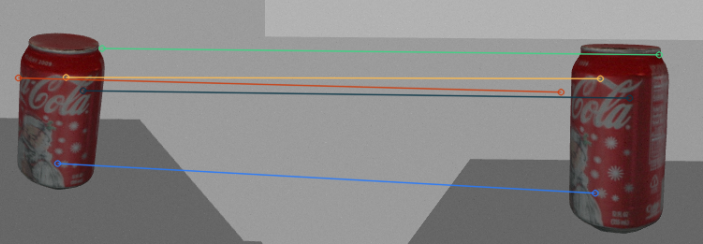
\includegraphics[width=0.7\textwidth]{query}
\caption{Matching finale tra i keypoints trovati dall'immagine proveniente dalla camera di sinistra ed i punti forniti per la fase di training.}
\label{fig:query_camera}
\end{figure}

\newpage

\subsection{\textit{move\_to\_object}}
Implementato nel file \textit{align\_to\_object.cpp} questo nodo si occupa della vera e propria esecuzione degli obbiettivi proposti gestendo le chiamate ai servizi di \textit{pose estimation}, \textit{robot controller} e ai metodi della classe \textit{Detector}. Esegue le seguenti operazioni:
\begin{enumerate}
\item Recupera i parametri intrinseci ed estrinseci delle due camere ed esegue la chiamata al servizio \text{InitCameras} fornendo oltre ai dati appena ricevuti i frame delle camere, end effector e robot base.
\item Chiama il servizio \textit{move\_robot} per spostare l'end effector nella posizione iniziale di training (Figura \ref{fig:train_pos}), questa sarà anche la posa goal che da raggiungere, nel caso no fosse raggiungibile lancia un messaggio di errore e ferma il programma.
\item Effetua una chiamata al metodo \textit{TrainMatches} della classe \textit{Detector} e passa i keypoints ottenuti in ingresso al servizio \textit{TrainPose} effetuandone la chiamata. Dopo vari tentativi si è notato che settando $kp\_num = 15$ e $max\_iteration\_number = 100$ fornisce i risultati migliori in termini di training della posa e velocità di esecuzione.
\item Recupera la trasformata dal Frame \textit{World} all'end effector (\textit{$ee\_link$}) e moltiplicandola per la rototraslazione ottenuta come risposta del servizio di training ottiene la trasformata dal sistema di riferimento \textit{\textbackslash world} alla posizione di goal; pubblica il dato appena trovato in ROS così da poter visualizzare il sistema di rifermento in $rviz$ (Figure \ref{fig:extr_poses} e \ref{fig:query_poses}).
\item Chiama il servizio $move\_robot$ per spostare l'end effector nella posizione di query. Se non è ragiungibile esegue un altro tentativo, nel caso anche questo non andasse a buon fine lancia un messaggio di errore e ferma il programma.
\item Effetua una chiamata al metodo \textit{QueryMatches} della classe \textit{Detector} iterativamente fino a che non riceve almeno 4 keypoints. Procedendo in modo analogo al caso precedente si è notato che settando $kp\_num = 20$ e $max\_iteration\_number = 100$ fornisce i risultati migliori in termini di corrispondenze trovate e velocità di esecuzione.
\item Converte la mappa di correlazione copiandone i dati in un vettore di numeri in formato \textit{long}, quindi passa in ingresso i keypoints ricavati al punto precendente, la mappa appena ottenuta e la camera da utilizzare al servizio \textit{QueryPose} effettuandone la chiamata.
\item In modo analogo a quanto visto nella fase di training calcola la trasformata dal Frame $world$ alla posizione restituita in uscita dal servizio \textit{QueryPose} e la pubblica in ROS così da avere un riscontro visivo in $rviz$.
\item se l'errore rispetto alla posizione di goal, sia per orientamento che posizione, è minore di $0.2$, oppure è minore rispetto all'iterazione precedente e non si sono verificati errori nella stima, sposta l'end effector nella posa appena calcolata chiamanto il servizio \textit{move\_robot}, altrimenti torna al punto (6).
\item Se l'errore in posizione è minore di $2cm$ ed in orientamento a $0.02$ la posizione di $Goal$ si considera raggiunta e termina l'esecuzione, altrimenti torna al punto (6). In Figura \ref{fig:end_pos} è rappresentata la posa finale ottenuta in una delle prove finali, come si può notare il frame desiderato coincide quasi perfettamente con quello stimato. Richiedere una precisione superiore può risultare controproducente in quanto non è detto che stime successive diano errori minori.
\end{enumerate}
Questo nodo può essere avviato attraverso il file \textit{find\_object.launch} nel quale si possono impostare diverse variabili che verranno passate al programma nella fase di avvio:
\begin{itemize}
\item Il path per l'immagine di template.
\item Il nome dei Frame delle camere, dell'end effector e della base del robot.
\item Il nome dei topics in cui vengono pubblicate le immagini ed i parametri dalle camere.
\item Il nome dei tre servizi forniti dal nodo di \textit{pose estimation}.
\item Le posizioni di train e query per l'end effector.
\item Ed infine il numero massimo di iterazioni ed il numero di keypoints per i due metodi \textit{TrainMatches} e \textit{QueryMatches} della classe \textit{Detector} e la telecamera da utilizzare nella fase di pose query.
\end{itemize}
Per la parte di pose query si è scelto di muovere l'end effector e non la lattina, in quanto in una applicazione reale il robot non conosce la posa dell'oggetto e non è quindi in grado di determinare l'errore tra la posa stimata e quella desiderata. Una soluzione potrebbe consistere nel calcolare lo spostamento tra due movimenti successivi e fermare la prova non appena questo scende sotto ad un certo valore. In questo modo non è però possibile trovare un bound fisso per l'errore finale, in quanto due prove successive $similmente$ sbagliate restituirebbero un movimento minimo in caso di posa sbagliata, rendendo più difficile valutare la qualità della prova stessa. I due metodi in ogni caso non differiscono, in quanto ad essere decisiva è solo la posa relativa in cui si trovano la lattina e l'end effector.

\begin{figure}[!ht]
\centering
\subfloat[Robot in posizione di \textit{train}.]	{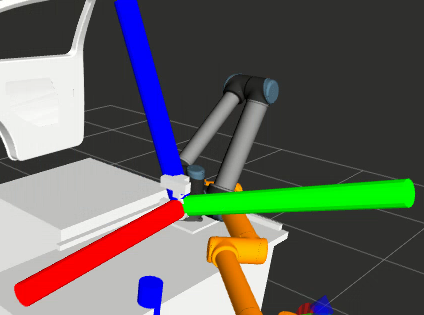
\includegraphics[width=0.43\textwidth]{train_pose}
\label{fig:train_pos}}
\subfloat[Robot nella posa stimata finale.]	{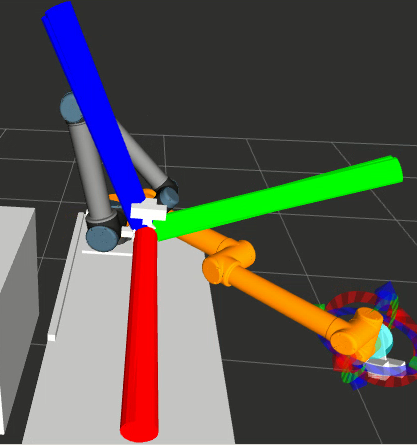
\includegraphics[width=0.3\textwidth]{end_pose}
\label{fig:end_pos}}
\caption{Confronto tra la posa di \textit{train} e la posa stimata finale con relativi piani di riferimento.}
\label{fig:extr_poses}
\end{figure}


\begin{figure}[!ht]
\centering
\subfloat[Robot nella prima posizione di \textit{query}.]	{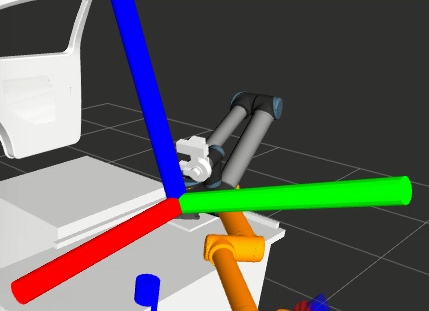
\includegraphics[width=0.38\textwidth]{query_pos_1}
\label{fig:query_pos1}}
\subfloat[Robot nella seconda posizione di \textit{query}.]	{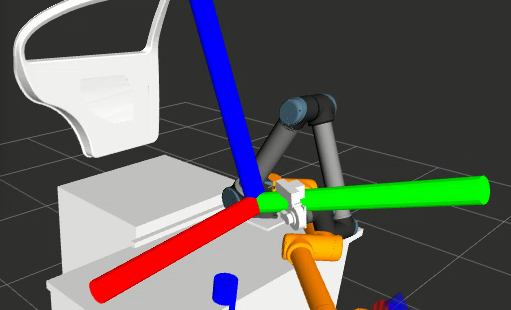
\includegraphics[width=0.45\textwidth]{query_pos_2}
\label{fig:query_pos2}}
\caption{Posizioni di \textit{query} del robot durante la prova e goal frame.}
\label{fig:query_poses}
\end{figure}

\section{Esecuzione}
Vediamo in questa sezione i comandi da inserire nel terminale per avviare l'esecuzione della prova. Innanzitutto si deve predisporre l'ambiente di simulazione nel quale verranno testati gli algoritmi. Il codice è stato testato in un laptop con sistema operativo Ubuntu 14.04 sul quale sono stati installati l'ambiente ROS indigo, i software forniti per l'esecuzione dell'esperienza ed il pacchetto da noi creato. Con i seguenti comandi, lanciati in sequenza da terminale, è possibile caricare il modello con il robot UR10 con giunti limitati:
\begin{verse}
\item $roslaunch \quad door\_assembly \quad simulation.launch limited:=true$
\item $roslaunch \quad ur10\_moveit\_config \quad ur10\_moveit\_planning\_execution.launch sim:=true$
\item 
\end{verse}
 A questo punto è dunque possibile avviare il path planner utilizzando il plug-in \textit{MoveIt!} e la visualizzazione della pianificazione in \textit{rviz} attraverso il seguente comando.:
\begin{verse}
\item $ roslaunch \quad ur10\_moveit\_config \quad moveit\_rviz.launch \quad config:=true $
\item 
\end{verse}
Una volta che l'ambiente di simulazione è stato avviato, è possibile aggiungere anche il modello dell'oggetto da identificare attraverso il sistema di visione, in questo caso una lattina. È possibile inserire tale oggetto, specificando le coordinate per ciascun asse cartesiano, attraverso il seguente comando. 
\begin{verse}
\item $rosrun$ $gazebo\_ros spawn\_model$ $-database$ $coke\_can$ $-sdf$  $-model$ $coke\_can$ -$y$ $0.3$ $-x$ $-0.2$ $-z$ $1.0 $
\item 
\end{verse}
\begin{figure}[!h]
\centering
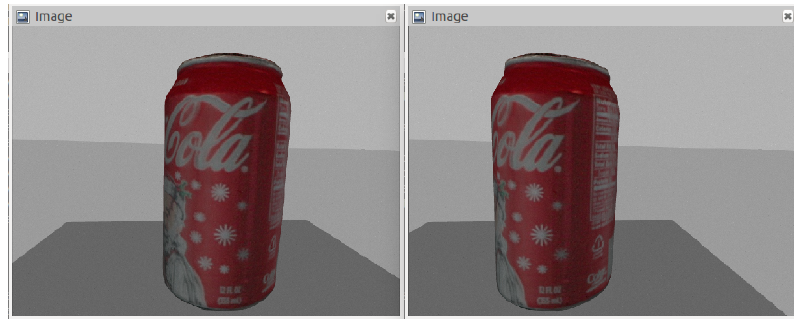
\includegraphics[width=0.5\textwidth]{coke}
\caption{Streaming video da entrambe le due telecamere in ambiente simulativo, fornito dal software \textit{rviz}.}
\label{fig:coke}
\end{figure}
In Figura \ref{fig:coke} è inoltre mostrato come sia possibile visualizzare l'oggetto creato, attraverso gli strumenti messi a disposizione da \textit{rviz}, nel caso particolare si è scelto di visualizzare lo streaming video delle due videocamere.
A questo punto è possibile avviare il nodo \textit{robot\_controller} che si occuperà di inizializzare il servizio per il movimento del braccio robotico:
\begin{verse}
\item $ roslaunch \quad  esperienza2 \quad robot\_controller.launch $
\item 
\end{verse}
Ora che tutto è pronto per l'inizio della prova, è sufficiente avviare il nodo \textit{find\_object}:
\begin{verse}
\item $ roslaunch \quad  esperienza2 \quad find\_object.launch $
\item 
\end{verse}

\section{Conclusioni}
A conclusione di questa esperienza, si sono dunque raggiunti gli obiettivi prefissati, il programma riesce a riposizionare il braccio nella posizione di train con buona accuratezza. Per validare il programma creato sono state registrate due intere prove di esecuzione in cui il robot si porta in due differenti pose di query riuscendo a raggiungere la posa desidera in meno di tre iterazioni in entrambi i casi. Alcune problematiche che si sono riscontrate riguardano il numero e la disposizione dei keypoints forniti al servizio \textit{QueryPose}, la stima va incontro ad errore se tra i keypoints forniti almeno quattro di questi non sono allineati o se se ne forniscono di meno. Di notevole importanza è anche la bontà dei matching tra i keypoints delle fasi di query e train, un solo match sbagliato porta ad errori consistenti. Infine la completa omogeneità del background nell'ambiente di simulazione può portare a falsi positivi negli algoritmi di matching in quanto non sempre si riesce ad avere una buona distinzione dei punti sui bordi della lattina. Per ovviare a questo problema nell'immagine di template (Figura \ref{fig:template}) si è scelto di utilizzare uno sfondo completamente nero.


\clearpage

\end{document}